%!TEX root = ../../Main.tex
\graphicspath{{Chapters/Teori/}}
%-------------------------------------------------------------------------------


\section{Color Sensor Module}
Color sensor modulet indeholder både en microcontroller og en color sensor. Til dette projekt har gruppen valgt at bruge en LC Technology TCS3200. Sensoren blev valgt fordi den var på lager i Embedded Stock, og at den ville passe godt til dette projekt. Til at styre denne sensor bruges en Arduino mega 2560.

\subsection{LC Technology TCS3200}
LC Technology TCS3200, virker ved at have 8x8 array af fotodioder. 16 fotodioder med et grønt filter, 16 fotodioder med et blåt filter, 16 fotodioder med et rødt filter og 16 fotodioder uden noget filter. De kan alle styres ved at sætte to pins(S2 og S3) høj eller lav. \cite{man:TC3200} Se \autoref{fig:PinSelect}

\begin{figure}[H]
	\centering
	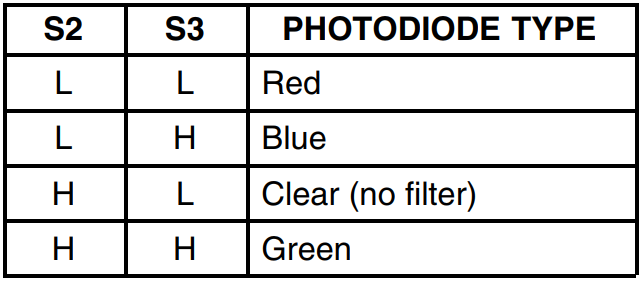
\includegraphics[width = 200pt]{Img/S1S2_color.png}
	\caption{Styring af photodioder}
	\label{fig:PinSelect}
\end{figure}

For at aflæse farveintensiteten, bliver man nødt til at måle på sensorens output pin. Signalet der kommer ud er et firkantssignal og farveintensiteten er bestemt alt efter hvor høj frekvensen er. For at se hvilken farve emnet har, bliver man nødt til at aktivere de forskellige fotodioder hver for sig, og tage en måling på output pin'en hver gang man har skiftet fotodiode. Derefter kan man så sammenligne de tre målinger (Clear bliver ikke målt) og se hvilket er størst. Hvis der skal måles andre farver end rød, grøn og blå, som fx gul, bliver man nødt til at kigge både på grøn og på rød. Hvis begge er lige høje må det være gul. Dog reagerer de forskellige fotodioder forskelligt på hvilken farve man ser på, så der skal der tages højde for. På \autoref{fig:FarveSpektrum} kan man se hvordan de forskellige fotodioder reagerer ved forskellige bølgelændger(farver)\cite{man:TC3200}.

\begin{figure}[H]
	\centering
	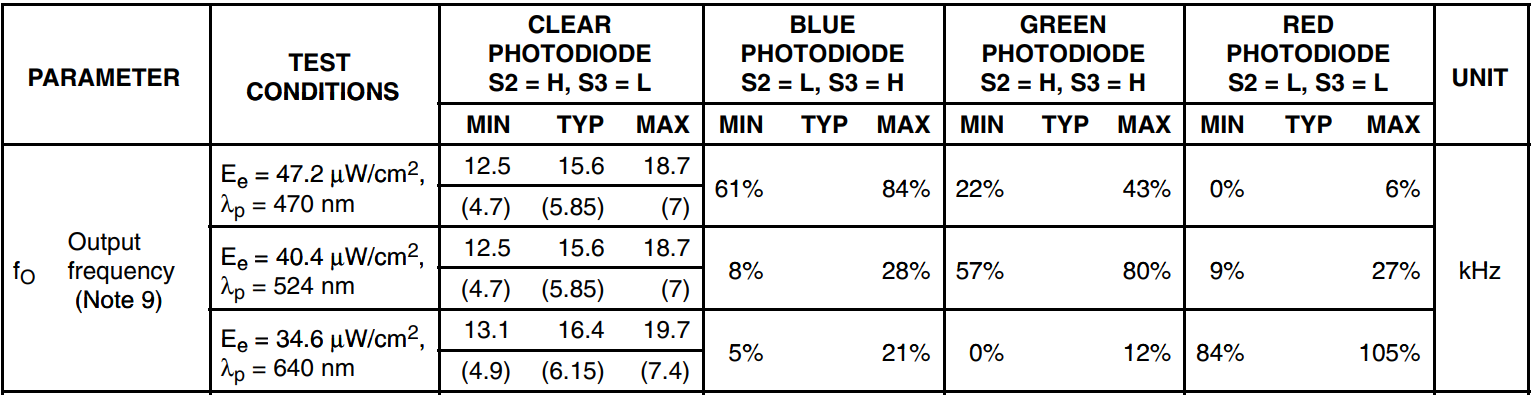
\includegraphics[width = 500pt]{Img/FarveSpektrum.png}
	\caption{Output frekvens ved forskellige farver}
	\label{fig:FarveSpektrum}
\end{figure}

En sidste ting der er værd er at vide om TCS3200, er dens indbygget frequency scaler. Den kan bruges til at styre skaleringen af output signalets frekvens. Skaleringen kan styres ved at sætte S1 og S2 høj eller lav. Til CSS bruges 2\% skalering, da 100\% skalering, ville betyde at output frekvensen kunne komme op over 50kHz. En lavere frekvens vil være fordelagtig i forhold til at få en præcis måling. \cite{man:TC3200} Se \autoref{fig:Frekvens}

\begin{figure}[H]
	\centering
	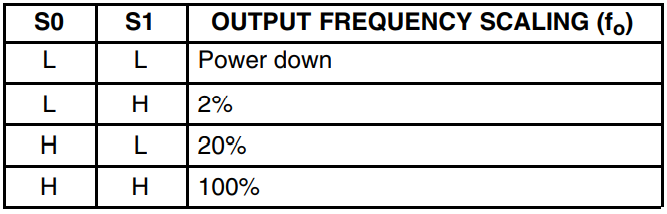
\includegraphics[width = 300pt]{Img/Frekvens.png}
	\caption{Output frekvens skalering}
	\label{fig:Frekvens}
\end{figure}

\subsection{Input Capture}
Input Capture er en metode der ofte bruges i embedded systemer, til at måle på diverse signaler. Til at måle outputsignalet fra TC3200 color sensor bruges denne metode.

\begin{figure}[H]
	\centering
	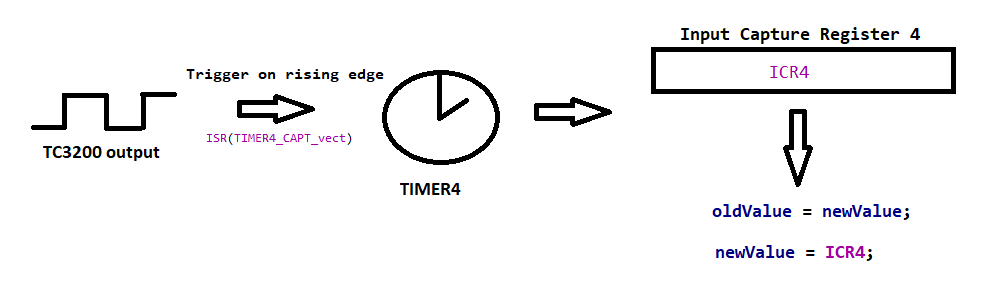
\includegraphics[width = 500pt]{Img/InputCapture.png}
	\caption{Input Capture illustration}
	\label{fig:InputCapture}
\end{figure}


Input Capture \cite{man:mega2560} fungerer ved at have et interrupt der trigger på rising edge. Når dette interrupt bliver kaldt, tages et øjebliksbillede af TIMER4s værdi, som gemmes i Input Capture Register 4. Denne værdi gemmes i en variabel, som bagefter bruges til at beregne en frekvens. 

Derudover skal der også tages højde for overflow, ellers kan man risikerer at en måling ikke vil give en korrekt frekvens. For at udbedre dette problem bruges en anden interrupt, ISR(TIMER4\_OVF\_vect). Den trigger hver gang der kommer overflow, og 65535 lægges til newValue. Koden til hvordan frekvensen udregnes kan ses nedenunder.

\newpage
\begin{lstlisting}
ISR(TIMER4_CAPT_vect)
{
	oldValue = newValue;
	newValue = ICR4;
	
	if(newValue < oldValue)
	{
		period = oldValue-newValue;
	}
	else
	{
		newValue + overflow;
		period = oldValue - newValue;
	}
	freq = F_CPU/period;
	FREQFLAG = 1;
}

\end{lstlisting}

Det kan også ses i koden, hvordan overflow værdien lægges til newValue, hvis newValue er mindre end oldValue. FREQFLAG bruges så man altid er sikker på at freq har en ny værdi. FREQFLAG skal selvfølgelig sættes til 0, når man har brugt freq.

\subsection{Color Sensor Module Software}
For nemt at kunne forstå softwaren brugt til TC3200, er der blevet udarbejdet et data flow diagram, der giver et overblik over dataflowet i softwaren. Dette diagram kan ses på \autoref{fig:DataFlow}. Som det ses i diagrammet, bliver der taget en frekvensmåling for hver farve. Dette gøres, som beskrevet tidligere, ved at sætte S2 og S3 enten høj eller lav. Når en måling er taget, sammenlignes de tre målinger for at se hvilken farve er mest repræsenteret. Derefter sendes en char som enten er 'R', 'G' eller 'B'. Kommunikationen sker via I2C. I2C vil blive uddybt mere i kommunikationsafsnittet. Derefter starter koden forfra igen, og tager en ny frekvensmåling. Source koden kan også ses under bilag.

\begin{figure}[H]
	\centering
	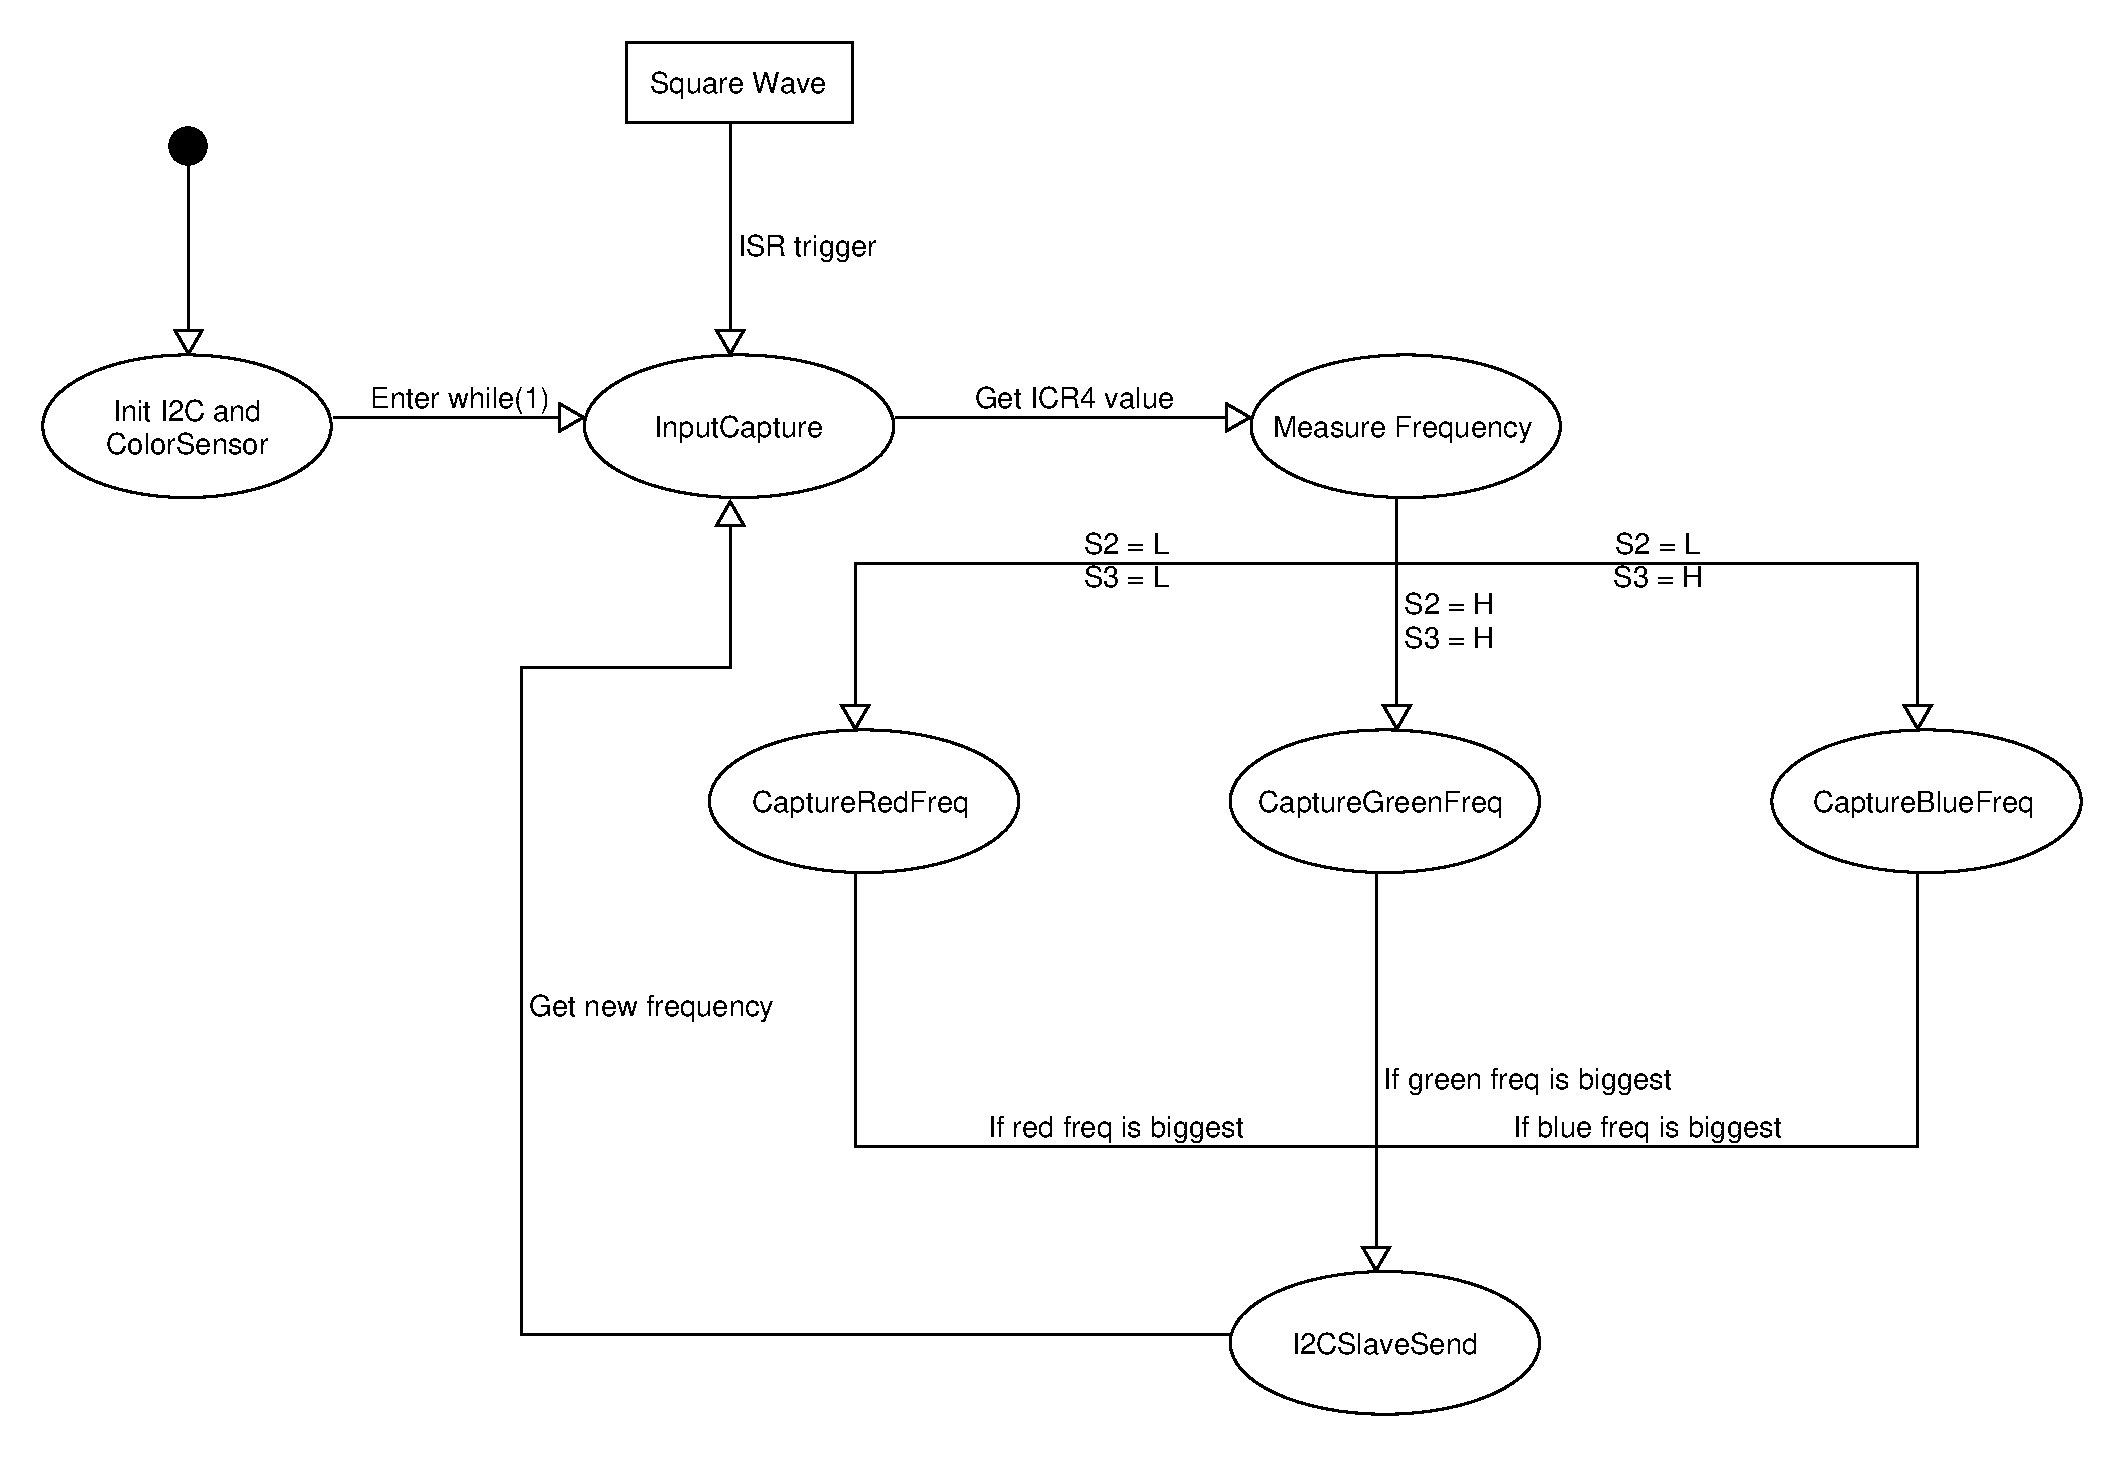
\includegraphics[width = 500pt]{Img/DataFlowDiagram.pdf}
	\caption{Data flow diagram}
	\label{fig:DataFlow}
\end{figure}


\subsection{Test}
En enhedstest er blevet lavet da modulet var færdigt. Resultatet af denne test vil bliver fremvist her. Først er input capture softwaren testet ved at bruge en funktions generator til at sende et firkantssignal ind på input capture pin'en. For at se om softwaren kunne aflæse den rigtige frekvens, er der gjort brug af UART kommunikation til en tilsluttet PC. Fra en terminal på PC'en har man kunne aflæse frekvensen fra arduino'en og derfra konstatere at programmet har virket.

\begin{figure}[H]
	\centering
	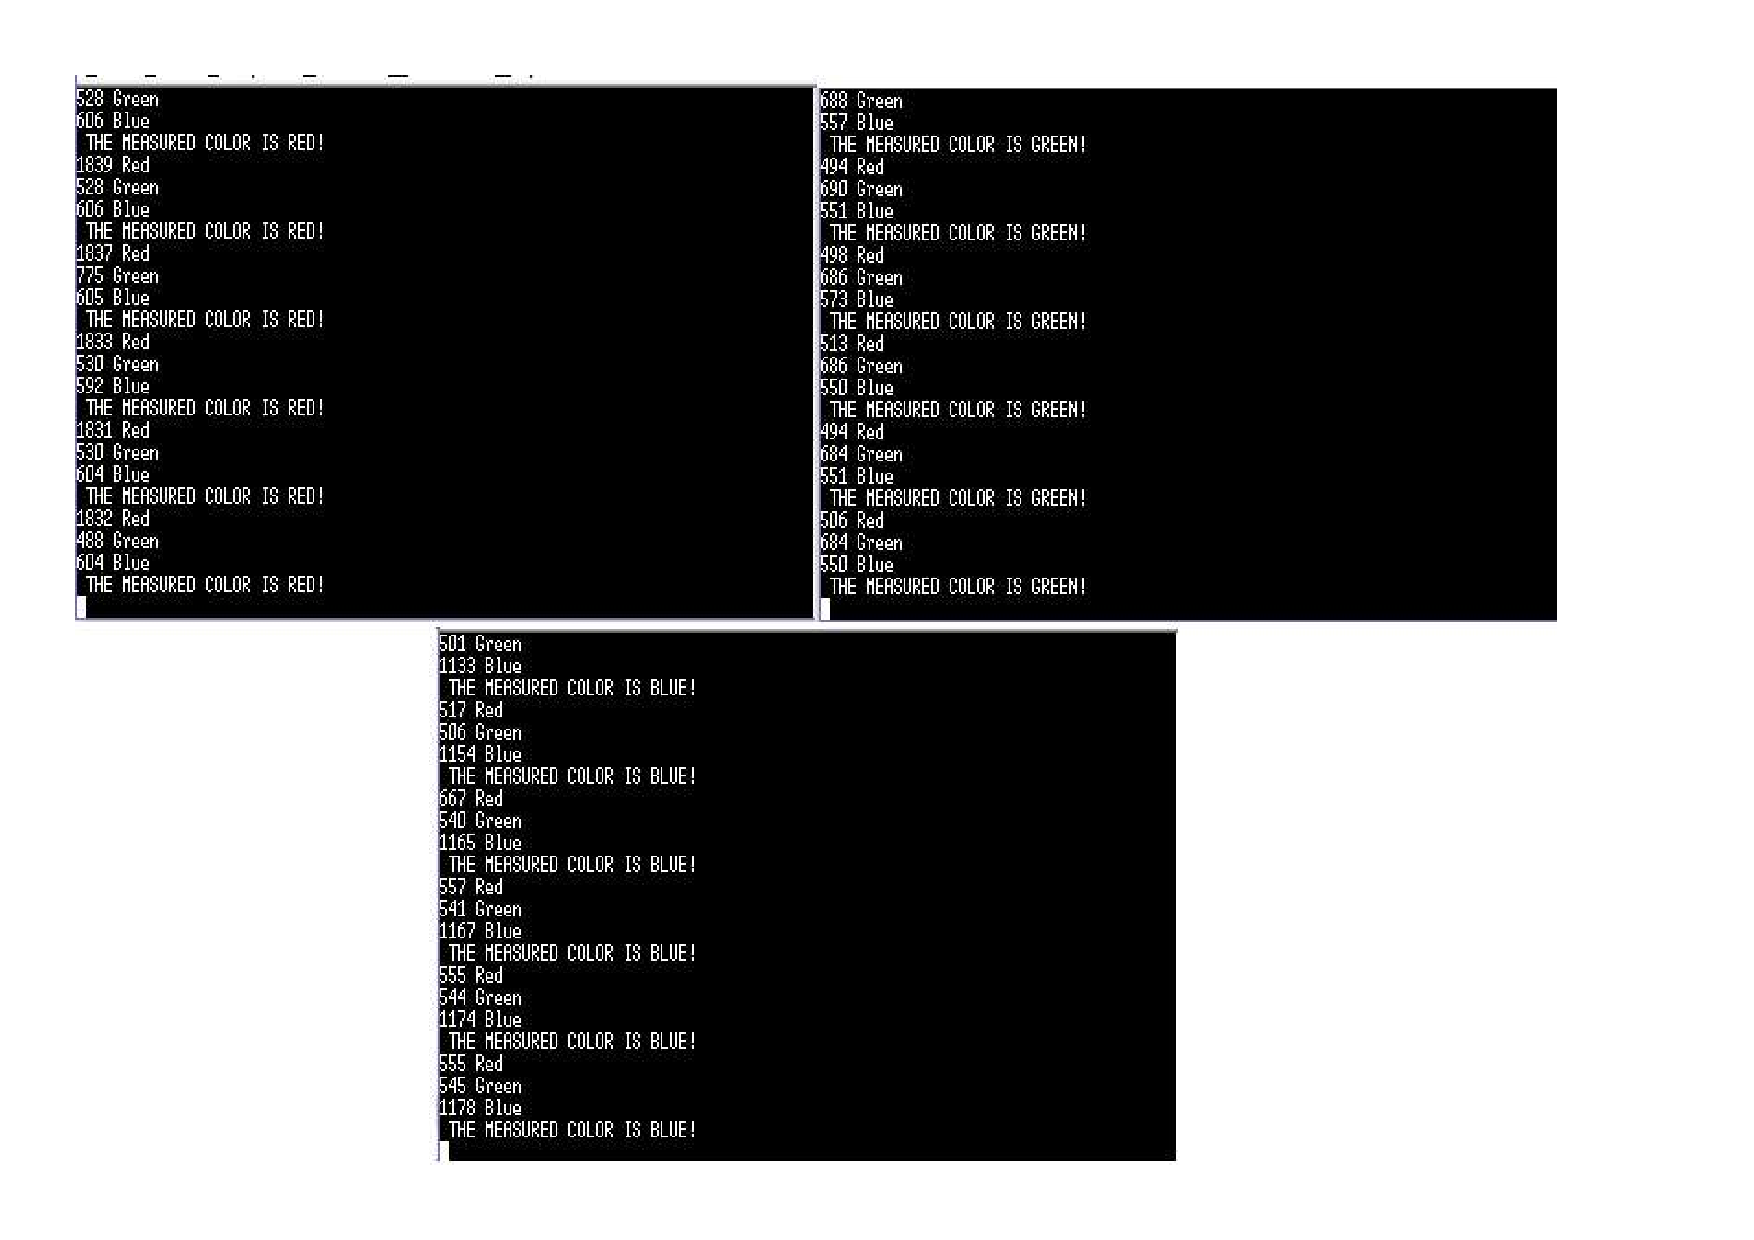
\includegraphics[width = 450pt]{Img/Test_all.pdf}
	\caption{Terminal output ved rød, grøn og blå test}
	\label{fig:Test_all}
\end{figure}

Til test af color sensoren, er der gjort brug af Input Capture programmet sammen med UART kommunikation til en PC. Sensorens output pin blev koblet til input capture pin'en, og tre målinger blev taget, én for hver farve(RGB). Farven med den højeste frekvens blev desuden sendt med som et bogstav, enten R B eller G. Som farvet forsøgsemne, blev tre forskelligt farvet stykker papir brugt. For at få så godt et resultat som muligt, skulle papiret holdes max 1cm fra sensoren, dog var det grønne papir stadig svært at opfange for sensoren. På \autoref{fig:Test_all} kan man se terminal outputtet fra sensoren. Tallene til venstre for "Red", "Green" og "blue" er frekvensen målt ved den farve. Man kan se hvordan sensoren har svært ved at opfange den grønne farve. Dette skyldes højst sandsynligt at farven ikke var den samme som databladet brugte til at teste med($\lambda = 524 nm$)\cite{man:TC3200}. Udover den grønne farve ikke passede helt, kan sensoren stadig skelne imellem de tre forskllige farver.

